\section{Our Solution}
\label{sec:rusc:solution}

Our solution is twofold. First, we develop a general and abstract
theory, called \emph{Refinement Under Self-related Contexts (RUSC)},
which is inspired by the standard notion of contextual refinement
\revision{and the notion of self-related context from \cite{stewart:ccc}
  (see \Cref{sec:related} for comparison).}
%\scc{}~\cite{?} (see \Sref{sec:related} for comparison).
Specifically, given a set of (arbitrary and independent)
relations each of which is horizontally compositional and adequate,
RUSC completes the relations by giving a super-relation (\ie
including all of them) that is horizontally and vertically
compositional and also adequate. Second, we prove that
our version of structured simulations, called \emph{open simulations},
with almost arbitrary memory relations
are horizontally compositional and adequate,
so that we can apply RUSC to open simulations with any chosen set of memory relations.

\myparagraph{Theory of RUSC}
%
RUSC can be defined abstractly for any linking algebra, which consists
of a set of modules, $\Module$, with a notion of behavior\footnote{Behaviors just need to be defined for closed programs.
  Technically, we can give undefined behavior (UB) to open modules.
%  For open modules, invoking an unknown function can be defined as undefined behavior (UB).
}, denoted
$\beh{p}$ for $p\in\Module$, a linking operation~$\llink$ between modules
that is associative%
\footnote{\revision{Commutativity does not hold for linking of \cc{} modules
    because changes in the order of global variables affect the initial memory after loading
    due to \cc{}'s deterministic memory allocation.}},
\revision{and the identity (\ie empty) module $\identity \in \Module$}:
\[
\begin{array}{c}
\llink: \Module \times \Module \rightarrow \Module \\
\forall p,q,r\in\Module,~p \llink (q \llink r) = (p \llink q) \llink r \\
\revision{\forall p \in\Module,~ \identity \llink p = p \llink \identity = p} \\
\end{array}
\]
Note that RUSC can be applied to interaction semantics because it
allows linking between arbitrary modules sharing the same notions
of value and memory (see \Cref{sec:overview-semantics:background} and \Cref{sec:main-semantics} for details).

To define RUSC, let $\rels$ be a set of module relations each of which is horizontally
compositional and adequate: for any $R \in \rels$ and $p,p',q,q'\in \Module$,
\[
\begin{array}{r@{}l@{\qquad}l}
(p,p'),(q,q')\in R &{}\implies (p \llink q, p' \llink q') \in R &\textrm{(\emph{HorComp})} \\
(p,p') \in R &{}\implies \beh{p} \supseteq \beh{p'} &\textrm{(\emph{Adequacy})} \\
\end{array}
\]
Then the RUSC relation for $\rels$, denoted $\rusc_{\rels}$, is defined as follows:
\[
\begin{array}{rcl}
p \rusc_{\rels} p' &\text{\emph{iff}}& \revision{\forall c_1, c_2 \in \self{\rels},~
\beh{c_{1} \llink p  \llink c_2} \supseteq \beh{c_{1} \llink p' \llink c_2}} \\
\self{\rels} & \defeq & \setof{ c \in \Module \suchthat \forall R \in \rels,~ (c,c) \in R }
\end{array}
\]
The definition is simple: $p$ is RUSC-related to $p'$ if the behaviors of $p'$ refine those of $p$ under
arbitrary contexts that are related to themselves by every relation in $\rels$.
% \jeehoon{From the definition of $p \rusc_{\rels} p'$, I think maybe it's easier to distinguish the
%   module type and the list-of-modules type... I know it's vague. Let's discuss offline.}

\begin{theorem}[Properties of RUSC]\label{thm:rusc} The RUSC relation $\rusc_\rels$ satisfies the following key properties.\\[.5mm]
$
\begin{array}{@{\quad}lrl}
 \text{(Inclusion)} &\forall R \in \rels,& R \subseteq {\rusc_\rels} \\[.5mm]
 \text{(Adequacy)} &\forall p,p'\in\Module,& p \rusc_{\rels} p' \implies \beh{p} \supseteq \beh{p'} \\[.5mm]
 \text{(VerComp)} &\forall p,p',p''\in\Module,& p \rusc_{\rels} p' \land p' \rusc_{\rels} p'' \implies p \rusc_{\rels} p'' \\[.5mm]
 \text{(HorComp)} &\forall p,p',q,q'\in \self{\rels},&   p \rusc_{\rels} p' \land  q \rusc_{\rels} q' \implies p \llink q \rusc_{\rels} p' \llink q' \\[.5mm]
 \revision{\text{(SelfComp)}} & \revision{\forall p,q \in \self{\rels},}& \revision{p \llink q \in \self{\rels}}
\end{array}
$
\end{theorem}
Note that horizontal compositionality holds only for self-related
modules, which, however, is not a big deal in practice as we will
discuss below.
\begin{proof}
The proof of the theorem is simple.  The
inclusion $R \subseteq {\rusc_\rels}$ trivially follows from the
horizontal compositionality and adequacy of $R$.  Adequacy of
$\rusc_\rels$ directly follows from the definition of $\rusc_\rels$ by
taking the empty context. Vertical compositionality (\ie transitivity)
of $\rusc_\rels$ holds trivially by definition.  Horizontal
compositionality, $p \llink q \rusc_{\rels} p' \llink q'$, is proven
in two steps using transitivity: $(i)$ $p \llink q \rusc_{\rels} p' \llink q$,
which follows from the definition of $p \rusc_{\rels} p'$ since $q\in\self{\rels}$,
and $(ii)$ $p' \llink q \rusc_{\rels} p' \llink q'$, which follows
similarly since $q \rusc_{\rels} q'$ and $p'\in\self{\rels}$.
%% ${R} \subseteq {\rusc_{\setofz{R}}}$ and
%% ${\rels} \subseteq {\rels'} \implies {\rusc_{\rels}} \subseteq {\rusc_{\rels'}}$
\revision{Finally, self-relatedness is closed under composition
because every relation in $\rels$ is horizontally compositional.}
\end{proof}

The reason why vertical compositionality is easily proven for RUSC
is that we essentially prove it for \emph{closed} programs by
closing an open module with contexts. Indeed, the technical
difficulties with vertical compositionality for open
simulations arise from the openness: it is difficult to set up a
setting properly with arbitrary future memories given after an external
function call.

The reason why horizontal compositionality holds between different
relations is interesting. Directly composing two simulations $(p,p') \in R_1$
and $(q,q') \in R_2$ with different relations $R_1$ and $R_2$
does not work in general. However, each simulation can be easily
extended with identical contexts because a pair of identical modules
usually respects any sensible relational principles. Therefore,
we have $(p \llink q ,p' \llink q) \in R_1$ and
$(p' \llink q ,p' \llink q') \in R_2$, which can be transitively composed
by vertical compositionality just as discussed above.
%% \jeehoon{I think we can say our horizontal compositionality proof, not the entire RUSC, is inspired
%%   from \scc{}.}

To sum up, RUSC provides a general condition for composing
different relational proofs: each proof just needs to be compatible
with its context modules in terms of self-relatedness, not necessarily
with their relational proofs.
%% instead of their relational proofs.

%% \begin{figure}
%%   \centering
%%   \includegraphics[width=0.70\linewidth]{rusc.jpg}
%%   \caption{Proving compositional compiler correctness with RUSC
%%   }
%%   \label{fig:rusc}
%% \end{figure}

%% \todo{add a fig:
%%   small horizontal compositionality figure,
%%   say that compatibility of rely/guarantee conditions between two relations (no)
%%   say that compatibility of rely/guarantee condition vs. the context I linked with. (yes)
%% }

\myparagraph{Open Simulations}
%
%% \todo{talk about analysis}
%% Since we can obtain vertical and horizontal compositionality
%% using RUSC, we can use simpler simulation relations (with different
%% memory relations)---which we call \emph{open simulations}---than
%% structured simulations (with structured injections).
%% Basically, open simulations contain only the core mechanism of
%% structured simulation presented in \Cref{sec:overview-verification:background}
%% without unnecessary complications needed to prove vertical
%% compositionality.

\revision{Since we can obtain vertical and horizontal compositionality using RUSC,
we can use open simulations with almost arbitrary memory relations.}
More specifically, we prove that open simulations with
\emph{any} Kripke-style memory/value relation satisfying certain minimal
conditions (see \Cref{sec:main-verification:parameter} for details) are horizontally compositional
and adequate. Since the required conditions are so minimal, they are
satisfied by the three memory relations---memory identity, extension
and injection---and also by a more powerful relation,
called \emph{memory injection with module-local invariants}.
This new memory relation is needed to
verify a new pass we added, called \texttt{Unreadglob}, which
requires reasoning about module-local states enabled by \emph{static}
variables of C (see \Cref{sec:overview-modulelocal} for details).

%% (emphasize that RUSC allows different techniques for different passes.
%% Additionally, analysis passes and assumptions on global variables).
Note that unlike \cc{} 2.1 on which \ccc{} is based, \cc{} 3.5
implements a static analyzer performing value analysis, which is used by
several passes. In order to support independent modular verification of such analyzers,
we also parameterize open simulations with memory predicates---representing the
analysis results of such analyzers---and
prove their horizontal compositionality and adequacy (See \Cref{sec:main-verification} for details).

\myparagraph{Applications} We use RUSC
% with open simulations
in two situations: compiler and program verification.
%% \jeehoon{On paragraph name: how about ``Applications''?  It sounds more general.}

First, we give an abstract example (presented in \Cref{fig:rusc-verif-scenario}) for compiler
verification.  Suppose our source program is written in three modules,
\texttt{a.c}, \texttt{b.c} and \texttt{c.asm}, and compiled via
multiple passes: $\texttt{a.c}\to\texttt{a.il1}\to\texttt{a.asm}$ and
$\texttt{b.c}\to\texttt{b.il2}\to\texttt{b.il3}\to\texttt{b.asm}$,
each of which is verified using a different relation $R_1$ to $R_5$.
\begin{figure}[t]
  \centering
  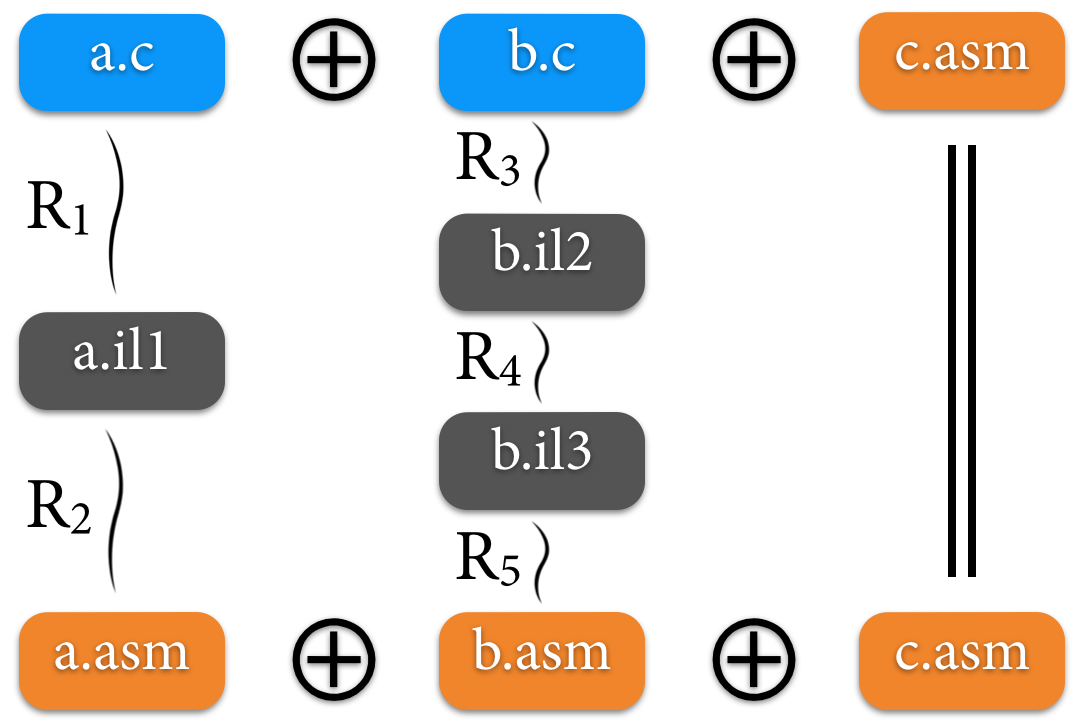
\includegraphics[width=0.90\linewidth]{images/fig-rusc.png}
  \caption{A compiler verification scenario with RUSC}
  \label{fig:rusc-verif-scenario}
\end{figure}
%
Then as long as the \emph{end modules}, \texttt{a.c}, \texttt{b.c}, \texttt{a.asm},
\texttt{b.asm}, \texttt{c.asm}, are self-related by the relations $R_1,\ldots,R_5$,
using RUSC we can obtain the following behavioral refinement:
\[
\beh{\texttt{a.c} \llink \texttt{b.c} \llink \texttt{c.asm}} \supseteq \beh{\texttt{a.asm} \llink \texttt{b.asm} \llink \texttt{c.asm}}
\]
The underlying reasoning is simple: for $\rels=\setof{R_1,\ldots,R_5}$, we get
\begin{itemize}
\item $\texttt{a.c} \rusc_\rels \texttt{a.asm}$ and $\texttt{b.c} \rusc_\rels \texttt{b.asm}$
  by Inclusion and VerComp of \Cref{thm:rusc};
\item $\texttt{c.asm} \rusc_\rels \texttt{c.asm}$ since
  %% $\texttt{c.asm} \in \self{\rels}$ and thus
  $(\texttt{c.asm},\texttt{c.asm}) \in R_1 \subseteq \rusc_\rels$
  by Inclusion of \Cref{thm:rusc};
  %% \jeehoon{I don't understand it..}
\item $\texttt{a.c} \llink \texttt{b.c} \llink \texttt{c.asm} \rusc_\rels \texttt{a.asm} \llink \texttt{b.asm} \llink \texttt{c.asm}$
  by HorComp of \Cref{thm:rusc};
\item $\beh{\texttt{a.c} \llink \texttt{b.c} \llink \texttt{c.asm}} \supseteq \beh{\texttt{a.asm} \llink \texttt{b.asm} \llink \texttt{c.asm}}$ by Adequacy of \Cref{thm:rusc}.
\end{itemize}
Note that we need to prove the self-relatedness only for the end
modules because we only link those, not the intermediate ones
like \texttt{a.il1}, \texttt{b.il2}, \texttt{c.il3}.
Moreover, proving self-relatedness by a relation is typically
straightforward as long as the relation is sensibly defined.  Indeed,
we could easily prove that \emph{all} Clight\footnote{Clight is taken
  as the source language in most verification projects using \cc{}
  such as VST~\cite{VST}, CertiKOS and even \ccc{}.
  However, we also prove behavioral refinement w.r.t. the C source language
  (see \Cref{sec:results}).
}
and assembly programs are
self-related by all the relations used by \ccm{}
(\ie open simulations with memory identity, extension,
and injection with or without module-local invariants).
%% \jeehoon{How about ``we could easily prove that \emph{all} C, Clight, ...''}

Second, we demonstrate, via small but interesting examples (see \Cref{sec:overview-modulelocal}),
% (see \Cref{sec:overview-modulelocal} and \Cref{sec:utod-verification}),
%% the possibility
that our framework can be used to verify program modules
against (open) mathematical specification modules, written in Coq's Gallina language.
In the above example, for instance, we can prove
\[
\begin{array}{c}
\texttt{a.spec} \rusc_\rels \texttt{a.c}\quad
\texttt{b.spec} \rusc_\rels \texttt{b.c}\quad
\texttt{c.spec} \rusc_\rels \texttt{c.asm}
\\
\texttt{abc.spec} \rusc_\rels \texttt{a.spec} \llink \texttt{b.spec} \llink \texttt{c.spec}
\end{array}
\]
and link them together with the compiler correctness results above to get
\[
\beh{\texttt{abc.spec}}
\supseteq %% \rusc_\rels
%% \texttt{a.spec} \llink \texttt{b.spec} \llink \texttt{c.spec}
%% \rusc_\rels
\beh{\texttt{a.asm} \llink \texttt{b.asm} \llink \texttt{c.asm}}
\]
as long as the mathematical specification modules \texttt{a.spec},
\texttt{b.spec}, \texttt{c.spec}, \texttt{abc.spec} are in $\self{\rels}$,
which is usually straightforward to prove.

\myparagraph{Comparison to Contextual Refinement}
%
As one can easily see, RUSC refines the standard notion of contextual
refinement: instead of quantifying over \emph{all} contexts, RUSC
quantifies over only \emph{self-related} contexts. The main difference
is that RUSC gives the notion of well-behaved context w.r.t. a given
set of program relations (\ie reasoning principles) in terms of
contexts self-related by them.  This is particularly useful when not
all contexts are well behaved.  For example, in the interaction
semantics allowing mathematical specification modules as above, one can
easily write a specification module that arbitrarily changes the whole
memory including other modules' private memory. Under the presence of
such ill-behaved contexts, the contextual refinement will end up being too
strong preventing any reasoning about private memory such as
functions' stack frames. On the other hand, RUSC w.r.t. a set of
sensible relations will rule out such bad contexts and give us a sensible (better) relation.
%% even in the presence of such ill-behaved contexts.


\myparagraph{Comparison to \scc{}}
\begin{figure}[t]
  \centering
  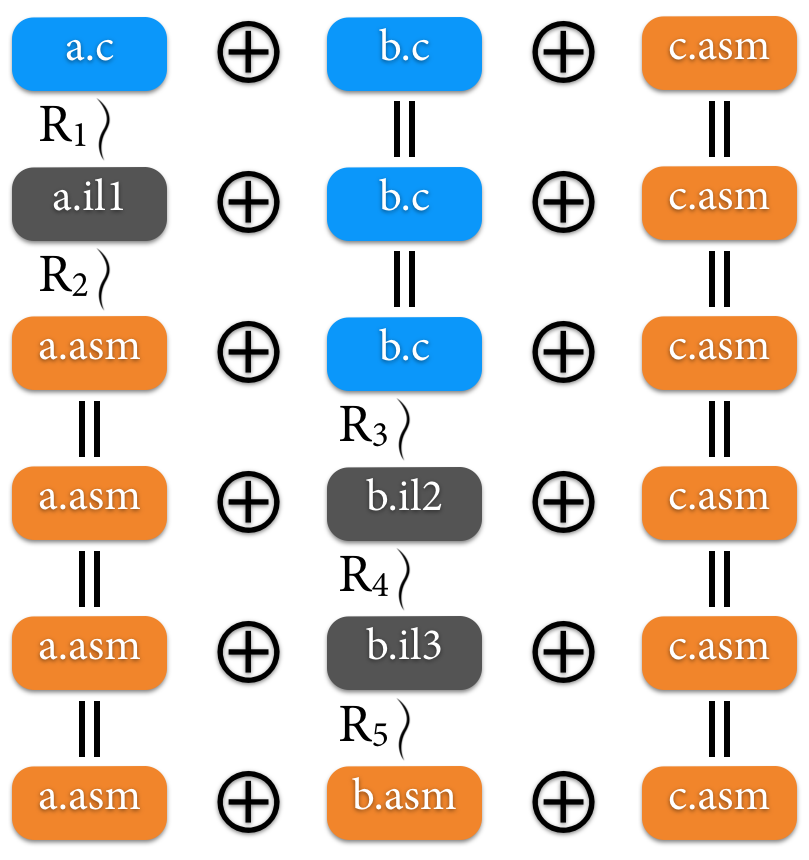
\includegraphics[width=0.90\linewidth]{images/fig-rusc-inline.png}
  \caption{An expanded version of the verification scenario described \Cref{fig:rusc-verif-scenario}}
  \label{fig:rusc-inline}
\end{figure}
If we ``unfold'' the notion of RUSC in the verification scenario above (\Cref{fig:rusc-verif-scenario}), what is happening under the hood is this: \Cref{fig:rusc-inline}.
Here, the key insight is that by inserting {\it dummy passes} -- which does not modify anything -- {\it only one} module is actually translated between each row.
Then, self-relatedness of \emph{end modules} and \emph{HorComp} and \emph{Adequacy} of each relation $R_i$ implies behavioral refinement between each row.
For instance, between the first and second row:
\begin{itemize}
\item $(\texttt{a.c}, \texttt{a.il1}) \in R_1$ is given;
\item $(\texttt{b.c}, \texttt{b.c}) \in R_1$ and $(\texttt{c.asm}, \texttt{c.asm}) \in R_1$ by self-relatedness of end modules;
\item $(\texttt{a.c} \llink \texttt{b.c} \llink \texttt{c.asm},\; \texttt{a.il1} \llink \texttt{b.c} \llink \texttt{c.asm}) \in R_1$ by \emph{HorComp} of $R_1$;
\item $\beh{\texttt{a.c} \llink \texttt{b.c} \llink \texttt{c.asm}} \supseteq \beh{\texttt{a.il1} \llink \texttt{b.c} \llink \texttt{c.asm}}$ by \emph{Adequacy} of $R_1$.
%% \item \beh{$\texttt{a.c} \llink \texttt{b.c} \texttt{c.asm}} $\supseteq$ \beh{$\texttt{a.il1} \llink \texttt{b.c} \texttt{c.asm}} by (\emph{Adequacy}) of $R_1$;
\end{itemize}

Actually, the idea of inserting dummy passes has already been employed in \scc{}'s ``Level B'' correctness, but their technique is akin to contextual refinement, and thus RUSC can be seen as a generalization of their technique.
Also, explicitly having a composable relation (RUSC) is both cognitively and technically useful.
Other minor differences are that in their setting, they used the syntactic linking operator $\plink$ concatenating modules of the \emph{same} language only, where our linking algebra allows language-independent linking.
Also, due to this restriction, \scc{} was able to use closed simulation while we use open simulation.

%% Most importantly, their approach is 
%% //비교: rusc notation 의 유용함, multi-language setting, open sim, ...

%% \begin{wrapfigure}{R}{1\linewidth}
%%\end{wrapfigure}


%% \myparagraph{Compositional Compiler Correctness}
